\newpage
\section{Aplikacja główna}
\paragraph{}
Glownym zalozeniem aplikacji w Unity jest stworzenie wirtualnego świata składającego się z wizualizacji dwoch scian oraz elementow znajdujacych sie na nich. Po wyznaczonych elementach poruszać się beda aktorzy, czyli postacie gry.

{\color{red}tutaj będą makiety}

\subsection{Świat gry}
\paragraph{}
{\color{red}Opisać}

\begin{center}
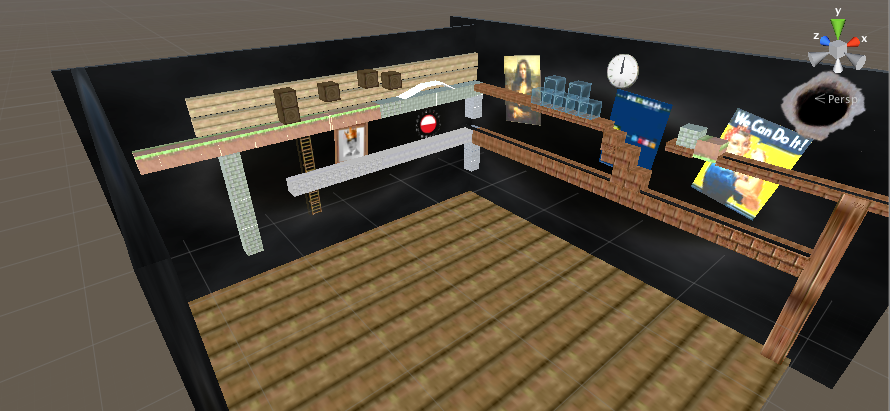
\includegraphics[width=0.9\textwidth]{images/swiatgry.png}
\captionof{figure}{
Model w środowisku Unity
}
\small {źródło: własne }
\end{center}


\subsection{Aktorzy}
\paragraph{}
{\color{red}Opisać}


\begin{center}

 \begin{tabular}{|c|c|}
 \hline  
  &   \\
  \hline   
  &   \\
  \hline   
\end{tabular}
\captionof{table}{Właściwości aktora}
\paragraph{}
{\color{red}Opisać}
\end{center}

\begin{lstlisting}[language=CSharp]
public void SendInfo() {
	Network.SendMessage("hasax_"+this.hasAx);
	Network.SendMessage("hassh_"+this.hasSh);
	Network.SendMessage("hasdrabina_"+this.drabina);
	Network.SendMessage("isMove_"+this.isMove);
}
\end{lstlisting}
\captionof{lstlisting}{
	Do Poprawy
}

\subsection{Prefabrykaty}
\paragraph{}
W Unity możliwe jest używanie prefabrykatów (Prefabs \footnote{http://docs.unity3d.com/Manual/Prefabs.html}). Są obiekty lub grupy obiektów, które służą do wielokrotnego wykorzystywania. W Projekcie założono, że wszystkie reużwalne komponety (dziedziczone pomiędzy scenami) będą prefabrykatami.

Dodatkowo aktorzy gry (generowane dynamicznie) są również prefabrykatami. Instancje aktora są tworzone podczas działania aplikacji.

\subsubsection{Kamery}
\paragraph{}
Ważnym elementem gry są wirtualne kamery. To z nich renderowane jest ujęcie, czyli obraz gry. W projekcie zastosowano dwie kamery. Podczas konfiguracji uruchomieniowej należy ustawić by każda z kamer była wyświetlana na oddzielnym źródle obrazu (monitor, projektor). Dzięki temu projekt można uruchomić na dwóch prostopadłych ścianach.
\paragraph{}
Jako tło sceny wybrano jednolity kolor czarny, ponieważ ten kolor nie jest prezentowany podczas projekcji. Światłó z projektora jest w tym miejscu znikome, wręcz niewidoczne. Stosując taki prosty zabieg można łączyć elementy rzeczywiste (np. rura czy inne elementy stałe znajdujące się w labolatorium) z wirtualną rzeczywistością.

\begin{center}
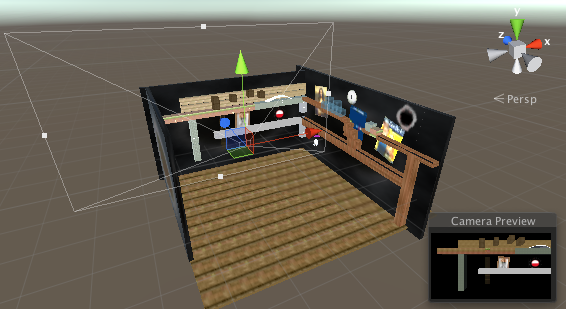
\includegraphics[width=0.9\textwidth]{images/kamera1.png}
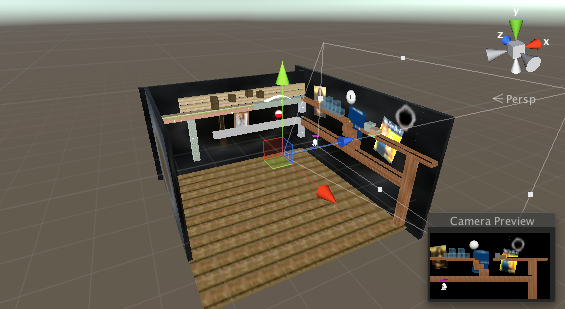
\includegraphics[width=0.9\textwidth]{images/kamera2.png}
\captionof{figure}{
Ujęcie wirtualnych kamer
}
\small {źródło: własne }
\end{center}

\paragraph{}
Środowisko Unity domyślnie nie ma włączonej opcji wspierania wielu kamer jednocześnie. Do opisywanego prefakbrykatu należy dodać abstrakcyjny GameObject z poniższym prostym skryptem, który przy uruchomieniu skopilowanej gry sprawdza dostępność sprzętową ekranów.

\begin{lstlisting}[language=CSharp]
using UnityEngine;
using System.Collections;

public class DisplayScript : MonoBehaviour
{
	void Start()
	{
		Debug.Log("displays connected: " + Display.displays.Length);
		if (Display.displays.Length > 1)
			Display.displays[1].Activate();
		if (Display.displays.Length > 2)
			Display.displays[2].Activate();
	}
}
\end{lstlisting}
\captionof{lstlisting}{
	Prosta aktywacja ekranów
}

\paragraph{}
Podczas testów uruchomieniowych przy dwóch kamerach występował problem z wydajnością karty graficznej. Zwłaszcza gdy do komputera podłączano dwa zewnętrzne ekrany po złączach cyfrowych (np. HDMI, DisplayPort, DVI). Finalnie problem rozwiązano wydajniejszym komputerem, jednakże pośredniom rozwiązaniem było użycie portu VGA, który jest mniej obciążający dla karty graficznej.

\subsubsection{Światło}
\paragraph{}
Kolejny prefabrykat stworzono by zachować spójność w oświetleniu trójwymiarowej sceny. Służy on do zgrupowania wszystkich źródeł wirtualnego światała. Jest to element bez zwwartej logiki biznesowej. Stworzono go w celu zachowania porządku w projekcie.


\subsection{SocketIO}
\paragraph{}
Jest to prefabrykat dostarczony jako kompotent implementacji Socket.io w bibliotece Asset Store. Jest on udostępniony na licencji Open Source.  Musi być on umiejscowiony w każdej scenie, która korzysta z połączenia sieciowego. Umiejscowienie jest dowolne, gdyż jest to prefabrykat abstrakcyjny (nie posiada graficznej reprezentacji w trójwymiarowym modelu). W prefabrykacie wywołano skrpyt SocketIOComponent, który odpowiada za inicjalizacje komunukacji sieciowej.

\subsubsection{Network}
\paragraph{}
Jest to kolejny prefabrykat abstrakcyjny, który służy do uruchomienia klasy Network odpowiadającej za implementacje metod służących do dwustronnej komunikacji.
Prefabrykat ten jest nierozerwalnie złączony z SocketIO, gdyż bezpośrendio korzysta z metod dostarczonych przez tą bibliotekę.


\begin{lstlisting}[language=CSharp]
private SocketIOComponent socket;

// Use this for initialization
void Start () {
	GameObject go = GameObject.Find("SocketIO");
	socket = go.GetComponent<SocketIOComponent>();

	socket.On("open", InitGame);
	socket.On("button", Button);
}
\end{lstlisting}
\captionof{lstlisting}{
	Inicjalizacja skryptu
}

\paragraph{}
Na początku wyszukiwaniy jest obiekt gry o określonej nazwie, a następnie pobierany komponent, czyli obiekt klasy. Warto pamiętać, ze połączenie inicjalizowane jest już przy uruchomieniu, więc nie ma potrzeby ,,ręcznego'' zestawiania warstwy sieciowej.

Metoda On w klase SocketIOComponent odpowiada za nasłuchiwanie serwera. Jako pierwszy parametr przymuje ciąg znaków określający nazwę metody. Natomiast drugi to referencja do metody, która wywoła się podczas wywołania akcji o nazwie wynikającej z pierwszego parametru.

Metoda zarejestrowana pod nazwą ,,open'' wywoła się przy udanym zestawieniu połączenia. Jest to najlepsze miejsce do wstępnej konfiugracji planszy gry oraz przycisków w kontrolerze.

{\color{red}Dokończyć opisywać logikę, network manager itd}.

\subsubsection{Replikator}
\paragraph{}
{\color{red}Opisać replikator}
\begin{center}
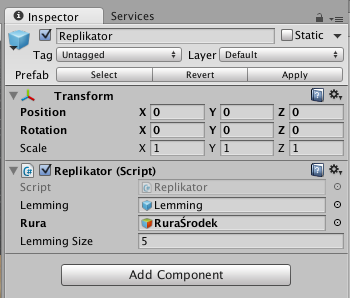
\includegraphics[width=0.7\textwidth]{images/replikator.png}
\captionof{figure}{
Konfiguracja replikatora
}
\end{center}

\begin{lstlisting}[language=CSharp]
...
public void Run () {
	StartCoroutine(Runner());

	NetworkManager.StartListening("button_left", Left);
	NetworkManager.StartListening("button_right", Right);
	NetworkManager.StartListening("button_kilof", Kilof);
	NetworkManager.StartListening("button_lopata", Lopata);
	NetworkManager.StartListening("button_jump", Jump);
	NetworkManager.StartListening("button_spadochron", Drabina);
	NetworkManager.StartListening("button_rotate", Rotate);
	NetworkManager.StartListening("button_startstop", Startstop);
	NetworkManager.StartListening("button_reset", Reset);
}

IEnumerator Runner() {
	while (lemmingCount < LemmingSize) {
		Create ();
		lemmingCount += 1;
		yield return new WaitForSeconds (secoundLimit);
	}
}
...
\end{lstlisting}
\captionof{lstlisting}{
	Uruchomienie replikatora
}

\begin{lstlisting}[language=CSharp]
...
void Left () {
	Lemming2.GetPrev ();
}

void Right () {
	Lemming2.GetNext ();
}

void Kilof () {
	if (Lemming2.activeEl) {
		Lemming2.activeEl.ToggleKilof ();
	}
}
...
\end{lstlisting}
\captionof{lstlisting}{
	Implementacja akcji
}


{\color{red}Opisać pozostałe prefabrykaty}

\subsection{Logika biznesowa}
\paragraph{}
{\color{red}Opisać}

\subsection{Serwer komunikacyjny}
\paragraph{}
{\color{red}Opisać}